% ST STEVAL-STWINBX1 node.
%
% Build:  make -C slides stwinbx1.pdf
% Figures: python3 slides/figures/make_kit_figures.py --kit stwinbx1

\documentclass[aspectratio=169,10pt]{beamer}
\usepackage{common/pdmtheme}
\graphicspath{{figures/}}

\title[STWIN.box node]{ST STEVAL-STWINBX1}
\subtitle{Wideband MEMS vibration node --- the reference kit}
\author{Predictive Maintenance Platform}
\date{13 October 2026}

\begin{document}

\begin{frame}[plain]
  \vspace{5mm}
  {\LARGE\bfseries ST STEVAL-STWINBX1}\\[2mm]
  {\large\color{pdmink2} Wideband MEMS vibration node}\par
  \vspace{5mm}\noindent{\color{pdmrule}\rule{\linewidth}{0.4pt}}\par
  \vspace{3mm}
  \begin{columns}[T]
    \begin{column}{0.46\textwidth}
      \scriptsize
      \kv{MCU}{STM32U585AI, M33 @ 160 MHz}\\[1mm]
      \kv{Vibration}{IIS3DWB, \textbf{6.3 kHz flat}, $\pm$16 g}\\[1mm]
      \kv{Acquisition}{8192 @ 26.667 kHz (307 ms)}\\[1mm]
      \kv{RAM used}{148 kB of 786 kB}\\[1mm]
      \kv{Radio}{BLE 5.2, 300 B frame}\\[1mm]
      \kv{Battery life}{\textbf{1.6 y as shipped, 15.2 y re-celled}}
    \end{column}
    \begin{column}{0.46\textwidth}
      \scriptsize\color{pdmink2}
      \textbf{Never flashed.} The shared DSP is verified against the Python
      reference (1\,113 C checks) and the application loop runs on the host, but
      no board has been on a bench. Timing and current figures are datasheet
      arithmetic.
      \\[2mm]
      \texttt{board\_stwinbx1.c} --- the IIS3DWB driver, DMA, clocks, BLE and
      sleep modes --- is the part that needs hardware.
    \end{column}
  \end{columns}
  \srcnote{Branch \texttt{hw/stwinbx1-stm32u5}. Detail:
    \texttt{hardware/stwinbx1/README.md}, \texttt{docs/hardware/stwinbx1.md}.}
\end{frame}

% ------------------------------------------------------------------ why ------
\begin{frame}{Why this part: bandwidth, not noise}
  \begin{columns}[T]
    \begin{column}{0.47\textwidth}
      \scriptsize
      \begin{tabular}{@{}lrrr@{}}
        \toprule
        & \textbf{IIS3DWB} & ADXL355 & ISM330BX \\
        \midrule
        Flat BW   & \textbf{6.3 kHz} & 1 kHz & 0.9 kHz \\
        Noise     & 75 & \textbf{25} & 70 \\
        \multicolumn{4}{@{}l}{\tiny $\mu$g/$\sqrt{\mathrm{Hz}}$} \\
        Full scale & $\pm$16 g & $\pm$8 g & $\pm$16 g \\
        Resolution & 16-bit & \textbf{20-bit} & 16-bit \\
        Current   & 1.1 mA & \textbf{0.2 mA} & 0.55 mA \\
        \bottomrule
      \end{tabular}
      \\[2.5mm]
      The ADXL355 is quieter and finer. The ESP32-S3 branch uses it for exactly
      that reason.
    \end{column}
    \begin{column}{0.49\textwidth}
      \small For bearing diagnosis, bandwidth wins.
      \\[1.5mm]
      \scriptsize
      A spalled raceway produces impacts at BPFO ($\approx$106 Hz here). The
      diagnostic information is \emph{not} at 106 Hz --- it is in the
      \textbf{modulation at 106 Hz of a structural resonance at 2--20 kHz}.
      \\[1.5mm]
      A sensor that rolls off at 1 kHz sees a rougher machine. It cannot see
      \emph{which} bearing element is damaged, no matter how low its noise
      floor.
      \\[2mm]
      And the IIS3DWB has exactly \textbf{one} output rate. No anti-alias filter
      to configure, no bandwidth/ODR ratio to get wrong, no mode where the part
      silently delivers less bandwidth than expected --- which on configurable
      parts is a common and nearly undetectable bug, because the data just
      looks smoother.
    \end{column}
  \end{columns}
  \takeaway{A magnet mount rolls off above $\sim$2 kHz and throws all of this
    away. Mount type is recorded per device for that reason.}
\end{frame}

% --------------------------------------------------------------- timing ------
\begin{frame}{The compute is not the problem}
  \centering
  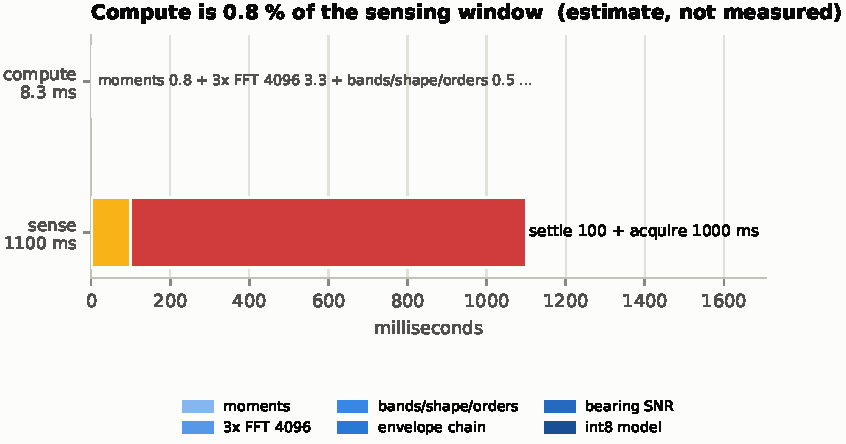
\includegraphics[width=0.74\linewidth]{kit_stwinbx1_timing.pdf}
  \\[2mm]
  \begin{columns}[T]
    \begin{column}{0.48\textwidth}
      \scriptsize
      8.6 ms of DSP against a 407 ms sensing window: \textbf{2.1 \%}. At one
      acquisition per hour that is a 2.4 ppm compute duty cycle.
      \\[1.5mm]
      So there is no case on compute grounds for the NPU- or Helium-bearing
      alternatives in this lineup. See the Alif branch for what an NPU actually
      buys, which is a \emph{bigger model}, not a faster one.
    \end{column}
    \begin{column}{0.48\textwidth}
      \scriptsize
      \textbf{Where the margin went instead.} 786 kB of SRAM is luxurious for
      this workload --- the pipeline uses 148 kB --- so this kit can afford a
      16384-sample acquisition (1.63 Hz envelope resolution) that the
      constrained kits cannot. It runs 8192 by default only for comparability
      across branches.
      \\[1.5mm]
      Substituting CMSIS-DSP's \texttt{arm\_rfft\_fast\_f32} is a one-line
      change --- the output packing convention is deliberately identical --- and
      should take $\sim$40 \% off the FFT line.
    \end{column}
  \end{columns}
\end{frame}

% --------------------------------------------------------------- energy ------
\begin{frame}{Where the energy actually goes}
  \centering
  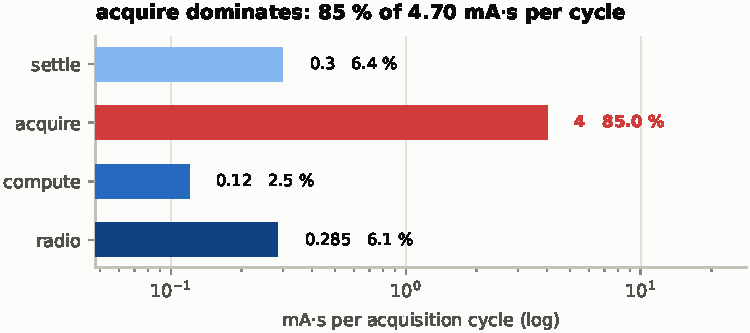
\includegraphics[width=0.66\linewidth]{kit_stwinbx1_energy.pdf}
  \\[1.5mm]
  \begin{columns}[T]
    \begin{column}{0.48\textwidth}
      \scriptsize
      \textbf{The acquisition window dominates: 85 \%.} Not the radio (6 \%),
      not the DSP (2.5 \%).
      \\[1.5mm]
      Most published vibration-node designs optimise the radio and the FFT. On
      this kit those are the two smallest terms. The levers that matter are a
      shorter record --- which costs envelope resolution --- and the IIS3DWB's
      1.1 mA operating current, which is fixed by the part.
    \end{column}
    \begin{column}{0.48\textwidth}
      \scriptsize
      \textbf{A 330$\times$ error this figure caught.}
      \texttt{APP\_SENSOR\_KEEPALIVE\_THRESHOLD\_S} was 90 s, on the stated
      reasoning that staying powered beats re-settling above that interval.
      Settling is 0.30 mA$\cdot$s once; keeping the sensor alive is 1.1 mA
      \emph{continuously}. The crossover is \textbf{0.27 seconds}.
      \\[1.5mm]
      At 90 s the node would have burned 99 mA$\cdot$s per cycle instead of 0.30
      --- battery life in weeks. Caught by a test that recomputes the crossover
      from the energy model rather than trusting the constant.
    \end{column}
  \end{columns}
\end{frame}

% -------------------------------------------------------------- battery ------
\begin{frame}{The cell, not the firmware, is the binding constraint}
  \centering
  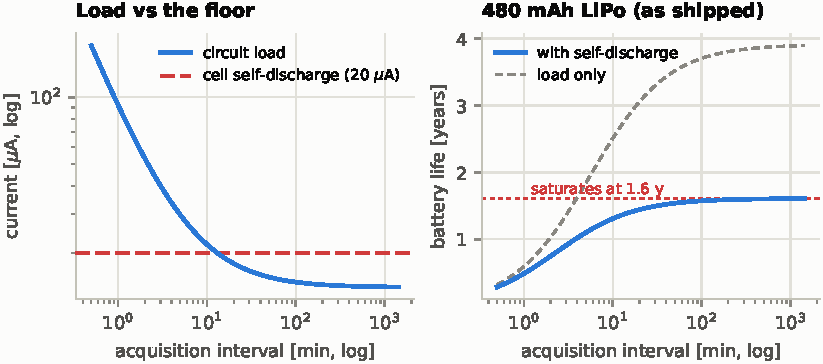
\includegraphics[width=0.70\linewidth]{kit_stwinbx1_battery.pdf}
  \\[2mm]
  \begin{columns}[T]
    \begin{column}{0.49\textwidth}
      \scriptsize
      The shipped 480 mAh LiPo self-discharges at 3 \%/month --- \textbf{20
      $\mu$A}, more than the circuit's 15.3 $\mu$A average draw. Battery life
      \emph{saturates at 1.6 years} regardless of interval; beyond $\sim$15
      minutes nothing the firmware does can improve it. The dashed curve is the
      circuit alone.
    \end{column}
    \begin{column}{0.49\textwidth}
      \scriptsize
      \textbf{Swap the chemistry:}
      \\[1mm]
      \texttt{\tiny power\_budget.py -\/-kit stwinbx1 \textbackslash}\\
      \texttt{\tiny ~~-\/-battery-mah 2400 -\/-self-discharge-pct-month 0.08}
      \\[1.5mm]
      $\Rightarrow$ \textbf{15.2 years}, with no firmware change.
      \\[1.5mm]
      LiSOCl$_2$ passivates after long storage and has a pulse-current limit
      that matters on the cellular kit --- but for a fit-and-forget vibration
      node it is the correct chemistry.
    \end{column}
  \end{columns}
\end{frame}

% ----------------------------------------------------------- limitation ------
\begin{frame}{The open metrological problem: $\pm$3 \% sample rate}
  \begin{columns}[T]
    \begin{column}{0.5\textwidth}
      \small
      The IIS3DWB's rate comes from an internal oscillator specified at
      $\pm$3 \%, and this board offers no way to measure the true value: the
      FIFO carries no timestamps at 26.667 kHz.
      \\[2mm]
      \scriptsize
      At the 3 \% extreme a 106.3 Hz BPFO line is computed as if it were at
      103.1 Hz. The matcher's $\pm$2 \% tolerance absorbs that --- just. By the
      \textbf{fifth harmonic} the error is 16 Hz against a $\pm$10.6 Hz window,
      so the top harmonics fall outside and \texttt{n\_matched} under-reports
      exactly when the evidence is strongest.
    \end{column}
    \begin{column}{0.46\textwidth}
      \scriptsize
      \textbf{Three fixes, one chosen}
      \\[1.5mm]
      \textbf{1. Reference tone at commissioning.} \textcolor{pdmgood}{Planned.}
      The self-test actuator produces a known mechanical deflection; drive it
      from an MCU timer and measure where the tone lands. Gives the true rate to
      0.02 \%. One extra second at commissioning, stored per device.
      \\[1.5mm]
      \textbf{2. Widen the tolerance to $\pm$4 \%.} Cheap and wrong: doubles the
      chance of matching a neighbouring family, which is what turns an
      inner-race diagnosis into an outer-race one.
      \\[1.5mm]
      \textbf{3. Track the 2$\times$ line-frequency component.} Free and as
      accurate as the grid --- but assumes the asset is mains-driven, false for
      anything on a VFD.
    \end{column}
  \end{columns}
  \takeaway{Until fix 1 ships, the firmware reports the nominal rate and the
    limitation is written down rather than hidden.}
\end{frame}

% ------------------------------------------------------------- unused --------
\begin{frame}{Two unused parts are more interesting than anything left to tune}
  \begin{columns}[T]
    \begin{column}{0.48\textwidth}
      \small\textbf{IMP23ABSU microphone, 80 kHz}
      \\[1.5mm]
      \scriptsize
      Complementary, not redundant. Needs \emph{no mechanical coupling}, so it
      sidesteps the mounting problem that dominates accelerometer practice --- a
      microphone hears a bearing through air where an accelerometer needs a stud
      into the housing.
      \\[1mm]
      80 kHz also reaches the low-ultrasonic band where lubrication distress
      appears earliest. The DCASE lineage in the research branch is built on
      exactly this signal, with a maintained MIT-licensed toolkit
      (\gh{TakuyaFujimura/dcase-asd-toolkit}).
      \\[1mm]
      The analogue output goes to the U5's ADC: firmware work, not hardware.
    \end{column}
    \begin{column}{0.48\textwidth}
      \small\textbf{ISM330BX MLC/ISPU as a wake-up filter}
      \\[1.5mm]
      \scriptsize
      85 \% of this kit's energy is the acquisition window. A decision tree
      running \emph{inside} the accelerometer on low-rate data, waking the MCU
      only when the vibration signature changes, attacks the dominant term
      directly. At long intervals the saving could be an order of magnitude.
      \\[1mm]
      The cost is a second model to train, validate and version --- and a new
      failure mode where the wake-up filter's false-negative rate silently
      becomes the system's detection limit.
      \\[1mm]
      Worth doing. Worth doing carefully.
    \end{column}
  \end{columns}
  \srcnote{Multi-axis is the obvious third option and is not obviously worth it:
    three axes triple the dominant energy term, and bearing faults rarely need
    an axial channel. Misalignment and looseness do.}
\end{frame}

\end{document}
